\documentclass{article}
\usepackage{graphicx}
\usepackage{listings}
\usepackage{hyperref}
\usepackage{pdfpages}
\usepackage{float}
\makeatletter
\newcommand\urlfootnote@[1]{\footnote{\url@{#1}}}
\DeclareRobustCommand{\urlfootnote}{\hyper@normalise\urlfootnote@}
\makeatother

\begin{document}
\title{Neural Networks Assignment 1}
\author{Oliver Scherp\\Matthias Mueller-Brockhausen}
\maketitle
\lstset{
  basicstyle=\ttfamily,
  keywordstyle=\bfseries,
  language=Java,
  frame=single,
  aboveskip=11pt,
  belowskip=11pt,
  breaklines=true,
  breakatwhitespace=false,
  showspaces=false,
  showstringspaces=false,
  numbers=left,
  stepnumber=1,    
  firstnumber=1,
  numberfirstline=true
}
\section{Excercise 1}
This is the table for our cloud distances.
The lowest and hence most similar values we found were 5.43, 6.01, 6.12 and 6.4.
These values were for classifying 7 to 9, 4 to 9, 3 to 5 and 9 to 8.
This does make sense given that a 9 can be, if written by hand, sometimes hard to distinguish from a 7, 4 or 5.


\section{Excercise 2}
The error rates we encountered were differnt to the ones expected. This can be explained by the amount of  actual numbers in the classified set.
Comparing the results of the training set classification (see Figure \ref{fig:cftrain}) against the test set classification (see Figure \ref{fig:cftest}).

\begin{figure}[H]
\centering
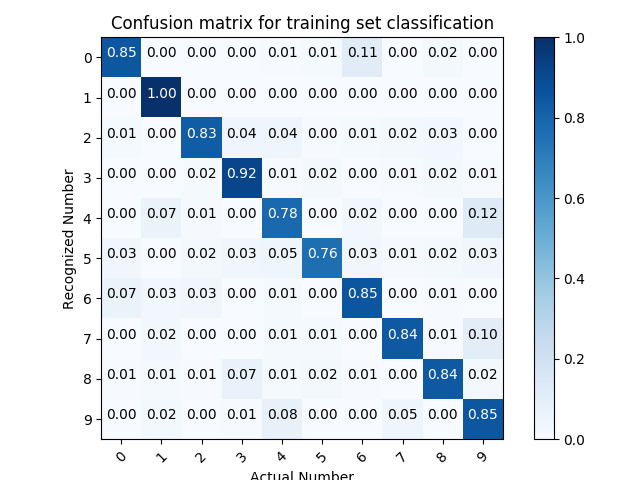
\includegraphics[width=0.9\linewidth]{img/cftrain.png}
\caption{Confusion Matrix visualized for Training Set}
\label{fig:cftrain}
\end{figure}
\begin{figure}[H]
\centering
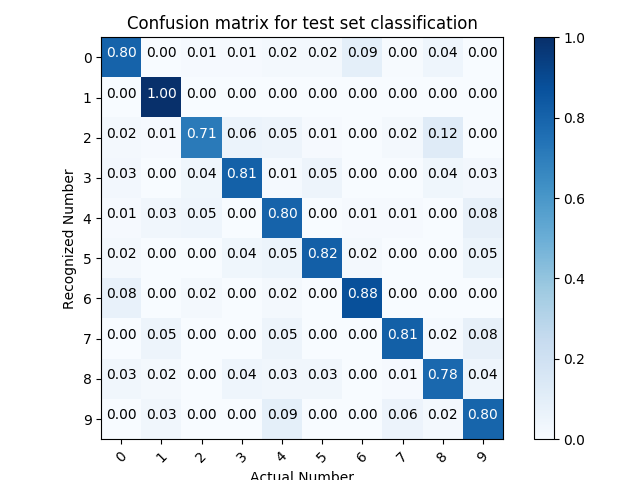
\includegraphics[width=0.9\linewidth]{img/cftest.png}
\caption{Confusion Matrix visualized for Training Set}
\label{fig:cftest}
\end{figure}



\end{document}